\chapter{Radio definida por Software}

Cuando en telecomunicaciones se habla de radio, se hace referencia al hardware necesario para transmitir o recibir información, haciendo uso de la banda del espectro radioeléctrico ubicado en radiofrecuencia (RF).

La mayoría de los sistemas de comunicación de hoy en día necesitan de un radio, la telefonía móvil,  la navegación por satélite, la aviación comercial, la televisión abierta, son todos ejemplos. En general los radios varían en dimensiones y costos según la aplicación, pero son muy poco versátiles en cuanto a sus capacidades. Con cada actualización tecnológica que reciben las redes, por ejemplo la modernización de la red móvil de 3G a LTE, implica una renovación total del equipamiento de radio. 

El concepto de Radio Definida por Software no es nuevo, algunas de sus ideas fundacionales se publicaron en la década de los 70. Pero ha sido el masivo desarrollo de la industria tecnológica el que ha impulsado en los últimos años la implementación de sistemas basados en SDR. 

Para implementar un equipo de radio definida por software, solo es necesario contar con una antena de radiofrecuencia, capaz de transmitir/emitir señales analógicas, y un conversor analógico-digital que alimenta de muestras a un procesador de propósito general. Es aquí donde radica la diferencia con los radios implementados en hardware, en los cuales se implementa toda una circuiteria electrónica para realizar el procesamiento. La masividad de los procesadores y el auge de la programación de hoy en día, permiten implementar fácilmente un SDR, y realizar todo tipo de proyectos de distinta escala, reutilizando el equipamiento. 

Durante la realización de este proyecto, utilizamos como entorno de desarrollo para crear los bloques de procesamiento de señales al software GNU Radio, y como antena utilizamos un equipo N200 del fabricante Ettus Research. 

\section{GNU Radio}

GNU Radio es un entorno de desarrollo orientado a procesamiento de señales, es gratuito y de código abierto. Mediante la interconexion de bloques de procesamiento, puede usarse en conjunto con antenas de RF para desarrollar SDRs, o en una versión local en modo de simulación de sistemas.
 
La aplicación por defecto trae una amplia gama de bloques funcionales para trabajar, desde herramientas simples como filtros y ecualizadores, hasta estructuras complicadas, como lo es un transmisor DTV completo.  Existe ademas una gran comunidad, muy activa, que esta permanentemente publicando nuevos contenidos, para ampliar la gama de herramientas existentes en la actualidad. 

Esto se da porque al ser de código abierto, es relativamente sencillo crear bloques nuevos. El entorno soporta desarrollos de código en python y en C++, siendo este ultimo el lenguaje con el que hemos implementado nuestro transmisor gr-isdbt-tx. Si bien puede parecer un poco complejo comprender la metódica de GNURadio en un principio,  una vez que comenzamos a trabajar con el y atravesamos la curva de aprendizaje, nos encontramos con una herramienta muy poderosa, y con la que es mas sencillo comprender algunos de los conceptos teóricos establecidos en la norma.
Durante la carrera, nos habíamos encontrado con GNU Radio en algunas ocasiones, donde pusimos en practica algunos conceptos básicos de sistemas de comunicación. No fue hasta esta instancia, en la que pudimos encontrarnos con el potencial total de la herramienta. 

Pasaremos a desarrollar algunos de los conceptos clave para comprender el uso de GNU Radio, ejemplificando con nuestro transmisor gr-isdbt-tx

\subsection{Flowgraphs}

El flowgraph es la estructura de datos mas básica del programa. Puede entenderse al mismo como si fuera una mesa de trabajo. Dentro de un flowgraph, vamos a insertar nuestras muestras desde la fuente, las vamos a procesar y las vamos a exportar, ya sea hacia un archivo o hacia el canal a través de una antena. 

\subsection{Bloques}

En GNU Radio, los datos siempre se mueven a través de bloques. Un bloque puede tener la fuente de datos, realizar operaciones sobre las muestras, puede exportar datos hacia el exterior del entorno, o puede tener toda una estructura de bloques adentro. 
Existen cuatro tipos de bloques, y de diferencian por la tasa de muestras que atraviesan el mismo. 

\textit{Bloques Sincronos (1:1)}, este bloque permite implementar funcionalidades que consuman y produzcan la misma cantidad de muestras por puerto. Los bloques sincronos pueden tener cualquier cantidad de entradas y salidas. En particular, cuando un bloque sincrono tiene 0 entradas, se tiene una fuente de datos (source). Cuando, al contrario, tiene 0 salidas, decimos que es un sumidero (sink). El bloque dispersor de energía por ejemplo, es un caso de bloque sincrono de gr-isdbt-tx. Volveremos sobre esto en el capitulo 5.

\textit{Bloques Decimadores (N:1)}, son los que producen menos muestras de las que consumen, y de forma análoga, existen también los \textit{Bloques Interpoladores (1:M)}.

Finalmente tenemos el caso general, \textit{Bloques Generales (N:M)}, en el cual no existe a priori una relación entre muestras de entrada y de salida, y cada usuario debe definirlo para el bloque en particular que esta creando mediante una función llamada forecast. Uno de los mas claros casos de bloque general en nuestro transmisor, es el bloque que crea el cuadro OFDM. En tiempo de compilación, no sabemos los parámetros de transmisión que determinan la tasa de muestras. Es en tiempo de ejecución que estos valores quedan definidos, el propio motor de GNU Radio se encarga de orquestar el flujo de datos para que todo funcione en régimen, 
Para implementar el transmisor, tuvimos que separar las funcionalidades en bloques de procesamiento, e implementar aquellos bloques que no estuviesen ya presentes en el repositorio. Algunos ejemplos como conversores serie a paralelo, el codificador Reed Solomon, el codificador Viterbi, existían ya como bloques funcionales del programa, y fueron re utilizados. 

\section{Hardware}
Universal Software Radio Peripheral (USRP) es una linea de plataformas de hardware para SDRs diseñados y comercializados por la empresa Ettus Research. Gran parte de la arquitectura de estos equipos es de código abierto, y puede ser descargada desde la web de la empresa. Con estos equipos se logra poner en funcionamiento soluciones de radio definida por software por costo accesible. 

En lineas generales, se componen de una placa madre en la que conviven varios subsistemas, como lo son un generador y sincronizador de señales de reloj, conversores analógico digitales y FPGAs, que se encargan de realizar tareas de procesamiento de señal en banda base. Se complementa con una placa modular de[h!]nominada “daugtherband” que realiza tareas como filtrado, condicionamiento de señal y modulación las señales en frecuencias de hasta 6 GHz.

\begin{figure}[h!]
	\centering
	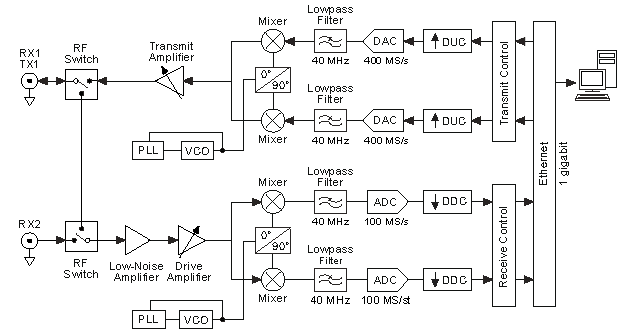
\includegraphics[scale=0.55]{figuras/cap04/usrp_arq}
	\caption{\label{f:usrp_arq} Arquitectura general de un equipo USRP}
\end{figure}

Durante este proyecto, trabajamos con el modelo USRP B100.

\subsection{USRP B100}

En este modelo, las muestras llegan al equipo a traves de una interfaz USB 2.0 y tiene una capacidad para transmitir en velocidades de hasta 16 MS/s, cuando se trabaja con muestras de 8 bits. 

Este modelo en particular esta actualmente discontinuado, pero su precio en el mercado rondaba los 700 dolares. Para el desarrollo del proyecto, recibimos en calidad de préstamo uno de estos equipos para las pruebas

Para poder levantar el equipo desde una PC, solamente es necesario instalar el driver universal de Ettus, “USRP Hardware Driver”. Con el driver instalado, es posible correr un analizador de espectro desde linea de comandos, para verificar que este funcionando correctamente.

\subsubsection{Interfaz con GNU Radio}

Para intercomunicar al equipo con el software de procesamiento de datos, es necesario incluir en el flowgraph, bloques de source o sink al equipo segun sea el caso. En gr-isdbt-tx, las muestras ya procesadas se enviaban al equipo a traves de un sink.  

\begin{figure}[h!]
	\centering
	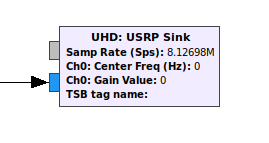
\includegraphics[scale=0.55]{figuras/cap04/sink_block}
	\caption{\label{f:sink_block} Bloque sink al equipo USRP}
\end{figure}

Los argumentos con los que funciona son la tasa de muestras, la frecuencia de destino en la que se desea transmitir y el valor de ganancia aplicado a la señal de entrada. 

A la hora de transmitir, es importante recordar algunas consideraciones con respecto al buen funcionamiento del equipo.

\section{gr-isdbt}